\clearpage
%%%%%%%%%%%%%%%%%%%%%%%%%%%%%%%%%%%%%%%%%%%%%%%%%%%%%%%%%%%%%%%%
\section{Introduction}
\setcounter{figure}{0}
\setcounter{table}{0}

%%%%%%%%%%%%%%%%%%%%%%%%%%%%%%%%
\subsection{L'observation directe des exoplanètes}
\label{sec:ImagerieDirecte}

%%%%%%%%%%%%%%%%
\subsubsection{Historique (\textit{intro sur l'etat de l'art, les parametres observés, atmosphère etc...})}
% imagerie indirecte a fait le plus de decouvertes
% ojd ~5000 exoplanetes decouvertes
% diagramme des exoplanetes decouvertes
% l'imagerie directe donne acces à une population différente d'exoplanètes
% cela permet des mesures photométriques et spectroscopiques donnant accès à l'atmosphère et la composition chimique de la planète
% il sera observé plutôt des systèmes jeunes car plus chaud et plus lumineux

%%%%%%%%%%%%%%%%
\subsubsection{La fièvre pour les techniques de coronographie}
% le principe de la coronographie
% liste des images d'exoplanètes

%%%%%%%%%%%%%%%%
\subsubsection{L'imagerie interférométrique}
% reconstruction par modèle
% astrométrie par ref de phase (reformuler pour titre)
% astrométrie par phase diff (reformuler pour titre)

%%%%%%%%%%%%%%%%%%%%%%%%%%%%%%%%
\subsection{L'imagerie haut contraste de systèmes exoplanétaires}

%%%%%%%%%%%%%%%%%%%%%%%%%%%%%%%%
\subsection{L'interférométrie}

%%%%%%%%%%%%%%%%%%%%%%%%%%%%%%%%
\subsection{Le masquage de pupille}
\label{sec:MasquagePupille}

%%%%%%%%%%%%%%%%%%%%%%%%%%%%%%%%
\subsection{Historique de l'instrument FIRST}

%%%%%%%%%%%%%%%%%%%%%%%%%%%%%%%%
\subsection{Les systèmes protoplanétaires}
\label{sec:Protoplanetes}

%%%%%%%%%%%%%%%%
\subsubsection{La formation planétaire}

La variété des exoplanètes jusqu'alors détectées permet d'étudier des conditions physiques, astrométriques et chimiques différentes, constituant une source d'informations pour la compréhension des systèmes planétaires. Notamment, leur évolution au cours du temps retient notre attention ici et est possible en étudiant différents systèmes d'exoplanètes se trouvant à différents stades de leur formation. 

Tout d'abord, l'étoile centrale se forme par effondrement de matière au sein d'un nuage de gaz, dominé par de l'hydrogène moléculaire. Lorsqu'un corps de quelques masses de Jupiter est formé, la densité y est suffisante pour qu'il y ait un état d'équilibre hydrostatique dans lequel la force de gravité compense la force de pression de la matière. Tout en s'effondrant sur l'étoile, le nuage de gaz acquiert un moment cinétique dominant et, en conséquence, se répartit sur un disque en rotation par effet centrifuge, ce qui explique que l'on retrouve les planètes et beaucoup de corps diverses du système solaire sur un même plan (l'écliptique). Ce disque protoplanétaire~\citep{williams2011} se forme rapidement, en moins de $10 \,$kyr et est à des températures telles qu'il est observable dans les grandes longueurs d'ondes millimétriques à infrarouge. La figure~\ref{fig:DiskEvo} est une schématisation des étapes majeures de l'évolution de ce disque. L'étoile est totalement formée en $0.5 - 1 \,$Myr et induit sur le disque des rayonnements \ac{UV} qui ont pour effet d'évacuer tout le gaz de la partie interne du disque vers les plus lointaines orbites en l'espace de $\sim 0.1 \,$Myr (figure~\ref{fig:DiskEvo} (a), (b) et (c)). Jusqu'à environ $10 \,$Myr, le disque est encore protoplanétaire et est optiquement épais (la lumière visible ne s'échappe pas de l'intérieur du disque). Il contient encore du gaz primordiale ainsi que de la poussière mais des intervalles vides se forment déjà, dû à la présence de protoplanètes. Entre $\sim 10 \,$Myr et $\sim 100 \,$Myr le disque est appelé disque de débris~\citep{wyatt2008} car il ne contient plus du tout de gaz, qui a été accrété par les planètes, et il est constitué de poussières de seconde génération, provenant des nombreuses collisions d'astéroïdes et de planétésimaux (figure~\ref{fig:DiskEvo} (d)). L'âge maximale typique d'un disque de débris est de quelques $100 \,$Myr. Il est possible d'étudier ces détails des systèmes planétaires via les mesures de leur spectre électromagnétique. En effet, selon la taille des grains de poussières (qui augmente avec le temps) le rayonnement détecté évoluera vers les courtes longueurs d'ondes. De plus, les disques protoplanétaires, dans leurs premiers stades d'évolution, sont optiquement épais et l'étude de la répartition spectrale d'énergie permet d'inférer dans quelle mesure le disque modifie le spectre de l'étoile centrale.

\begin{figure}[ht!]
    \centering
    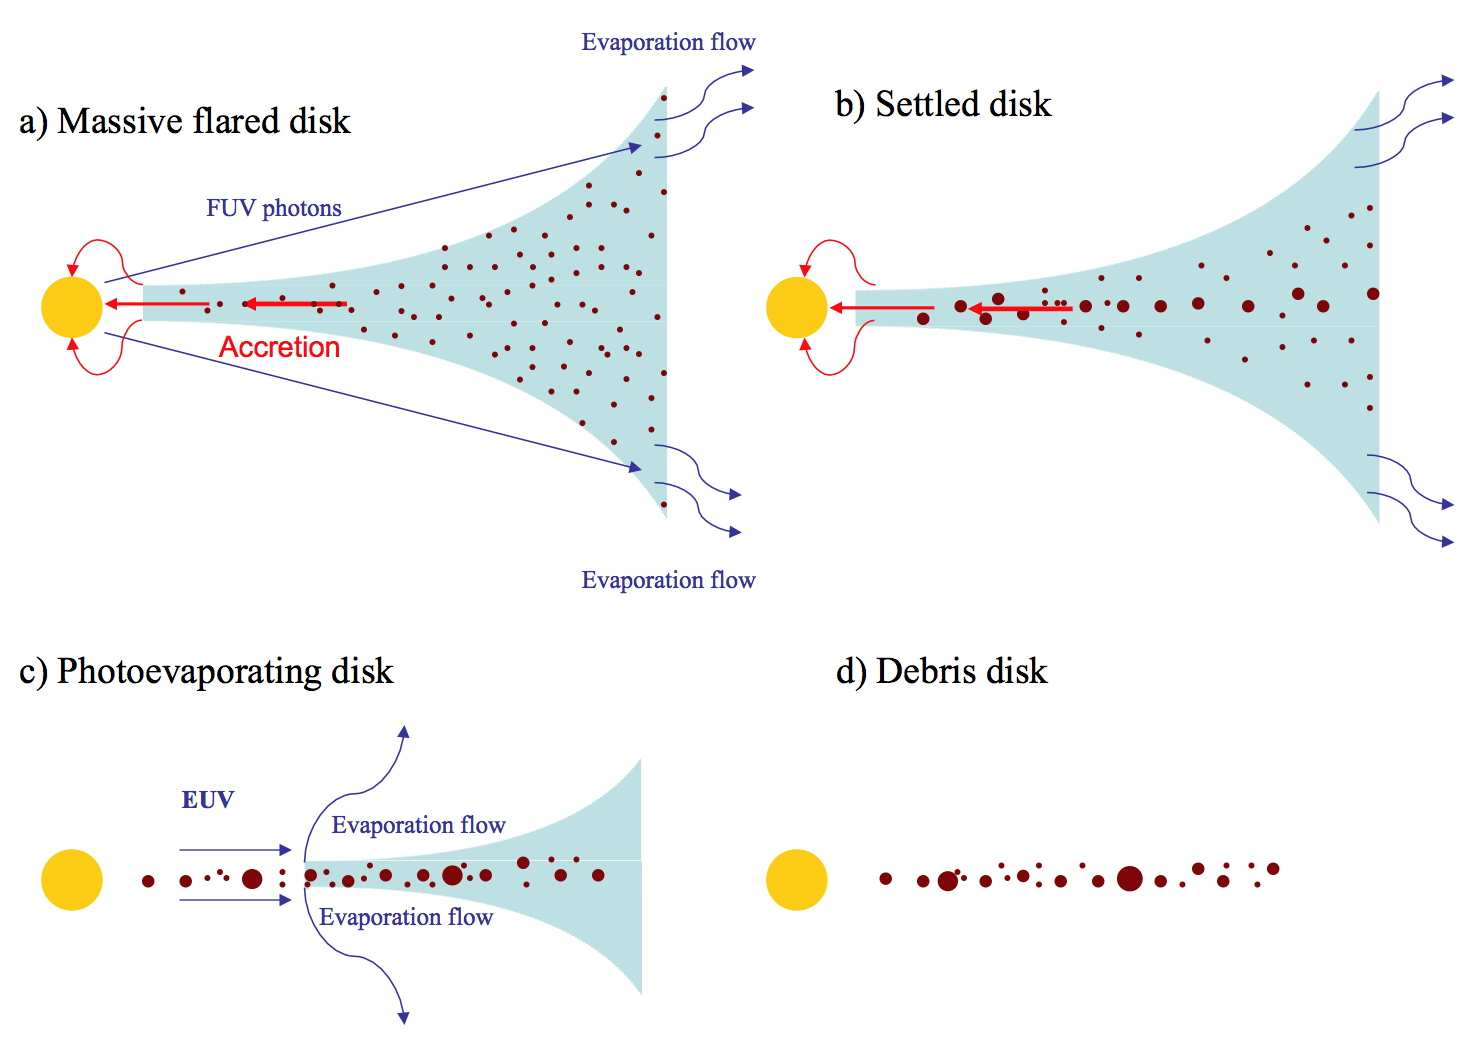
\includegraphics[width=\linewidth]{Figure_Chap1/Williams2011_Fig06_PlanetaryDiskEvolution.png}
    \caption[Évolution typique d'un disque protoplanétaire.]{Évolution typique d'un disque protoplanétaire, tiré de~\cite{williams2011}. Le gaz est représenté en bleu et les poussières en marron. (a) Le disque dans son stade d'évolution primitif ($0-1\,$Myr) perd de la matière par accrétion sur l'étoile et photo-évaporation par les rayonnements \ac{UV} émis par l'étoile. (b) Les grains de poussières s'agglomèrent en débris de plus en plus gros tout en se répartissant sur un même plan. (c) L'étoile a finis de se former et le disque interne est dépourvu de gaz, devenant optiquement fin en quelques $0.1 \,$Myr. (d) Les plus petits grains de matières se font soit retirer par pression de radiation soit sont accrétés par les planètes et il ne reste que les planétésimaux au sein du disque, qui devient de plus en plus difficile à détecter, en l'espace de quelques $100 \,$Myr.}
    \label{fig:DiskEvo}
\end{figure}

Dans le même temps, on identifie $3$ stades d'évolutions des exoplanètes observées, pendant lesquels les exoplanètes sont nommées :

\begin{enumerate}
    \item protoplanètes lorsque le système est âgé de moins de $4 \,$Myr, ce sont les exoplanètes qui m'intéressent dans le cadre de mon projet de thèse, elles sont toujours en formation et accrètent de la matière, au sein du disque protoplanétaire et ont une forte émission dans la raie \ha~(comme on le verra plus en détails dans la section~\ref{sec:AccretionAlpha});
    \item jeunes planètes géantes lorsque le système est âgé de $4 \,$Myr à $100 \,$Myr, sont au sein d'un disque de débris, elles n'accrètent plus de matière mais ont une température assez élevée ($\sim 700 - 1700 \,$K) pour émettre un rayonnement thermique visible et infrarouge et font partie du groupe d'exoplanètes les plus détectées en imagerie directe (e.g. Beta Pictoris b~\citep{lagrange2010});
    \item planètes complètement formées lorsque le système est âgé de plus de $100 \,$Myr, constituant la grande majorité des exoplanètes connues et sont trop froides pour avoir une émission thermique comme sur les deux types d'exoplanètes précédemment cités, mais peuvent refléter suffisamment la lumière de leur étoile pour être détectées en imagerie directe.
\end{enumerate}

À ce jour, deux grandes théories existent pour décrire les mécanismes de formation planétaire. La première théorie est la formation par accrétion de matière (\ac{CA}, en anglais), pour la première fois énoncée dans~\cite{safronov1972}. Les grains de poussières microscopiques se combinent pour former des corps de plus en plus gros : des astéroïdes, puis des planétésimaux (future planète). Enfin, si ces corps ont une masse d'au moins $10 \,$ M$_{\bigoplus}$, ils accrètent du gaz et deviennent des géantes gazeuses~\citep{pollack1996}. Pour le système solaire, cela explique donc bien la présence de quatre planètes rocheuses dépourvues de gaz car il a été expulsé par le Soleil (comme expliqué dans le paragraphe précédent) sur les plus petites orbites ainsi que de planètes géantes gazeuses sur les orbites les plus lointaines et dont on soupçonne qu'elles contiennent un noyaux rocheux.

Bien que cette première théorie est la plus acceptée par la communauté, notamment pour expliquer la formation du système solaire, de récents travaux montrent qu'une deuxi\hyp{}ème théorie est plausible. Cette théorie fait appelle à des processus d'instabilités gravitationnelles (\ac{GI}, en anglais) et est, par exemple, simulée dans~\cite{nayakshin2017}. Ici, juste après la formation de l'étoile, des régions localisées dans le disque exoplanétaire se condensent par instabilités gravitationnelles en des corps de plusieurs fois la masse de Jupiter. Dans ces conditions, les grains de poussières sédimentent et forment un noyaux rocheux central. Certaines simulations~\citep{boley2010} montrent que ces amas se formant à $\gtrsim 50 \,$AU et migrent jusqu'aux basses orbites ($\sim 1 \,$AU), où ils perdent leur couche de gaz à cause des effets de marrés (\ac{GI}). Cela réussit aussi à expliquer la présence de petites planètes rocheuses aux orbites les plus proches du Soleil et des géantes gazeuses dotées de noyaux rocheux sur des orbites plus éloignées, où les effets de marrés ne sont pas suffisamment forts pour dissiper leur gaz.

Il est probable que les mécanismes de ces deux théories soient à l'oeuvre au cours de la formation planétaire. L'étude d'un plus grand nombres de systèmes protoplanétaires est donc indispensable pour contraindre ces théories.


%%%%%%%%%%%%%%%%
\subsubsection{L'accrétion de matière des protoplanètes}
\label{sec:AccretionAlpha}

Comme nous l'avons vu dans la section~\ref{sec:ImagerieDirecte}, l'imagerie directe permet l'étude de systèmes exoplanétaires encore jamais étudiés et permet une étude photométrique et spectroscopique de ceux-ci. Cette technique est adaptée à l'observation de protoplanètes car d'une part ce sont des systèmes jeunes et chauds donc très lumineux et d'autre part elle permet la mesure d'observables directement liées aux processus de formation planétaire.

L'une de ces observables qui nous intéresse est le spectre d'émission. En effet, l'accrétion de matière par un astre induit l'émission de raies associées à l'hydrogène dans le spectre mesuré. Lorsque le gaz, principalement composé d'hydrogène s'effondre sur une étoile ou une planète, il atteint des vitesses qui dépassent la vitesse du son locale. Le gaz génère en conséquence des ondes de choc augmentant la température de plusieurs milliers à plusieurs dizaines de milliers de Kelvins. À cette température, l'hydrogène est excité et émet les raies spectrales des bandes Lyman, Balmer, Paschen, etc. Ces émissions ont été simulées pour des proto-étoiles jeunes en accrétion à partir de modèles d'accrétion magnétosphérique~\citep{muzerolle2001, natta2004, espaillat2008}, dans lesquels le gaz interagit avec le champ magnétique stellaire et permettant ainsi de déterminer les liens entre ces émissions le taux d'accrétion. De telles émissions hydrogènes ont été mesurées pour un échantillon d'étoiles jeunes du nuage Lupus~\citep{alcala2014, alcala2017}, permettant d'estimer leur taux d'accrétion de matière ainsi que les liens entre la géométrie des flux d'accrétion et le taux d'accrétion. Une étude similaire sur le taux d'accrétion de l'étoile PDS70 a aussi été conduite dans~\cite{thanathibodee2020} en utilisant un modèle d'accrétion magnétosphérique. PDS70 est dites de type T Tauri (\ac{TTS}, en anglais)~\citep{appenzeller1989}, qui définis les étoiles variables jeunes en formation, âgées de moins de $10 \,$Myr et appartenant à la pré-séquence principale (ici PDS70 est de type spectrale K7). Comme beaucoup d'étoiles de type \ac{TTS}, PDS70 est dotée d'un disque de transition (stade d'évolution entre le disque protoplanétaire et le disque de débris). Ces disques se caractérisent par la présence d'orbites pratiquement vides contenant parfois des protoplanètes. Les taux d'accrétion ont plusieurs fois été calculés pour les étoiles de type \ac{TTS}~\citep{natta2004, rigliaco2012, ingleby2013}.

Ces modèles d'accrétion de matière, initialement développés pour des étoiles jeunes et peu massives, ont été adaptés pour le cas de protoplanètes~\citep{aoyama2018, thanathibodee2019}. Les difficultés d'une telle adaptation sont que les conditions d'accrétions sur les protoplanètes sont différentes de celles sur les étoiles : dans le cas des protoplanètes, (1) la température du gaz en accrétion est moins élevée (d'au moins un ordre de grandeur), (2) le milieu dans le voisinage de la protoplanète (le disque circumplanétaire) n'a pas les mêmes structures (c'est parfois un bras de gaz et de poussière~\citep{boccaletti2020} approvisionnant en matière l'étoile) et (3) les champs magnétiques locaux sont différents en intensité et en structure, entraînant des écoulements de gaz différents dans l'un ou dans l'autre des cas. Plus simplement, dans le cas des étoiles, le gaz est excité avant le choc supersonique et est ionisé après le choc car les champs magnétiques locaux sont assez puissants pour accélérer les écoulements alors que dans le cas des protoplanètes, le gaz n'est excité seulement qu'après le choc supersonique~\citep{aoyama2019}.

L'étude des raies d'émissions hydrogène de Balmer, plus particulièrement la raie Balmer-$\alpha$ ($656.28 \,$nm), aussi appelée raie \ha, est un bon moyen d'estimer le taux d'accrétion de matière en cours sur les protoplanètes~\citep{aoyama2019, marleau2022}. \ac{FIRSTv2} est conçu pour travailler dans cette gamme de longueur d'onde et ainsi détecter une raie \ha. C'est pour cela que dans la suite, je vais m'intéresser essentiellement aux travaux effectués sur la détermination du taux d'accrétion à partir de la mesure de cette raie.

Il est possible de contraindre le taux d'accrétion de matière de plusieurs manières différentes :

\begin{itemize}
    \item soit par l'utilisation de modèles magnétosphériques d'accrétion~\citep{natta2004, ingleby2013, thanathibodee2019}, de modèles hydrodynamiques d'écoulement du gaz lorsqu'il s'effondre sur la protoplanète~\citep{aoyama2018, aoyama2019, aoyama2020} ou de modèles d'émission par un bloc d'hydrogène à certaines conditions de température et de pression~\citep{alcala2017, rigliaco2012}. Ces modèles sont ajustés aux spectres mesurés pour inférer la luminosité des raies d'émission ou directement la luminosité d'accrétion $log(L_{acc})$, qui sont alors utilisées pour calculer le taux d'accrétion avec les méthodes énoncées au point suivant.
    
    \item Soit par la mesure de l'intensité du pic \ha~qui permet de déduire la luminosité \ha~émise par la protoplanète connaissant sa distance à la Terre. Pour des étoiles de faibles masses ($< 0.1 \, M_{\odot}$), comme celles de type \ac{TTS}, la luminosité $log(L_{\text{\ha}})$ est reliée à la luminosité d'accrétion $log(L_{acc})$ par une relation affine selon $log(L_{acc}) = b + a \times log(L_{\text{\ha}})$. Enfin, le taux d'accrétion $\dot{M}$ est proportionnelle à la luminosité $L_{acc}$ libérée à l'impacte du flux d'accrétion sur la surface du corps selon une équation de chute libre provenant du modèle d'accrétion magnétosphérique~\citep{gullbring1998}. \cite{wagner2018} applique cette méthode sur le système PDS70 et \cite{rigliaco2012} l'applique sur un échantillon d'une dizaine d'étoiles de type \ac{TTS} pour plusieurs raies d'absorptions de l'hydrogène. Il propose ainsi d'étalonner la relation entre l'émission \ha~et le taux d'accrétion pour ce type d'étoiles afin d'être employée à l'avenir sur le même type d'objet~\citep{close2014}.
    
    \item Soit par la mesure de la largeur du pic \ha~émis. Plus précisément, de la largeur du pic à $10 \, \%$ de sa hauteur (W$_{10}$) qui est élargie en fonction du taux d'accrétion. En effet, \cite{natta2004, fang2009} suggèrent un seuil indiquant que des cibles qui présentent une largeur W$_{10}$ du pic \ha~inférieur à $4.4 \,$\AA (ou $200 \,$km.s$^{-1}$) n'accrètent pas de matière, dans le cas de corps de faibles masses de type stellaire (\ac{CTTS} ou \ac{WTTS}) ou géantes gazeuses. C'est aussi ce que montre les simulations de~\cite{thanathibodee2019} (figure 4b) pour les protoplanètes du système PDS70 : il existe un seuil en dessous duquel (W$_{10} = 100 \,$km.s$^{-1}$) la largeur de l'émission \ha~ne dépend pas du taux d'accrétion $\dot{M}$ pour $\dot{M} < 10^{-8} \,$M$_{\text{Jup}}$.yr$^{-1}$. Les valeurs de seuil de taux d'accrétion diffèrent selon ces études car les modèles de simulations utilisés sont appliqués dans les premiers cas pour des corps stellaires de faibles masses et dans le deuxième cas pour des protoplanètes. Mais encore, le taux d'accrétion des protoplanètes du système PDS70 a pu être calculé à partir des largeurs W$_{10}$ mesurées sur les spectres obtenus sur l'instrument MUSE~\cite{haffert2019, hashimoto2020}.
\end{itemize}

L'intérêt d'étudier les protoplanètes dans la raie \ha~est que le contraste de luminosité planète / étoile est bien moins élevé (d'un facteur $50$ à  $1000$ selon~\cite{close2014}) ce qui augmente les chances de détection par \ac{FIRSTv2}. La mesure d'une telle raie permettrait à la fois de discriminer la présence d'une protoplanète qui, dans le reste de la bande spectrale, serait en dehors de la gamme de performances de l'instrument; mais aussi d'étudier son taux d'accrétion.

Dans les cas précédemment cités où le flux de la raie d'émission est utilisé, le taux d'extinction devra, dans certains cas, être pris en compte. En effet, étant donné que les protoplanètes se trouvent dans un disque de gaz et de poussières, ce dernier atténue son flux lumineux d'un facteur $A_R$. Pour le système PDS70, par exemple, la limite basse de ce taux a été estimé à $2.0 \,$mag et $1.1 \,$mag, respectivement pour la planète b et la planète a~\citep{hashimoto2020}. Cette estimation a été faite à partir de modèles d'hydrodynamique simulant la quantité d'hydrogène moléculaire qui peut être liée à l'extinction de la poussière interstellaire. Ce taux d'extinction en \ha~de l'émission mesurée d'une protoplanète se fait donc en se basant sur nos connaissances du système, notamment sur la présence de gaz et de poussières (qui diffère pour un disque de transition par rapport à un disque plus jeune sans transition) qui peut être inféré par l'étude des spectres du système à d'autres longueurs d'ondes.

Il est aussi intéressant de noter que ce facteur d'extinction n'affecte que la hauteur des pics d'émissions et non leur largeur. On voit donc ici l'intérêt d'être capable de mesurer la largeur du pic \ha, notamment la largeur à $10 \, \%$ de la hauteur W$_{10}$, qui peut ainsi se faire sans se soucier de l'extinction au sein du disque. Mais pour cela, il est nécessaire de disposer d'une résolution spectrale suffisante. Par exemple, la raie spectrale mesurée sur PDS70b~\citep{haffert2019} a une largeur à mi hauteur égale à FWHM$\, = 0.27 \pm 0.03 \,$nm et on souhaite mesurer six points sur cette raie, correspondant à un élément de résolution de $\delta\lambda = 0.09 \,$nm. Cela nécessite un spectrographe avec une résolution spectrale à $656.28 \,$nm de R$\, = 7292$. Actuellement, la résolution spectrale du spectrographe de \ac{FIRSTv2} est de R$_{FIRSTv2} = 4000$ (section~\ref{sec:InstruSpectro}) et ne permet donc pas de mesure fiable de la largeur d'une raie d'émission \ha~mais seulement sa mesure d'intensité.

Actuellement plusieurs systèmes semblent être pourvus de protoplanètes, entre autres : 

\begin{itemize}
    \item les deux protoplanètes mises en évidence~\citep{keppler2018, muller2018} autour de l'étoile PDS70, déjà mentionnée plus haut, qui présentent une émission \ha~plusieurs fois mesurée et étudiée. Je les présenterai plus amplement dans la section~\ref{sec:pds70}.
    
    \item Le système LkCa 15 présentant 3 protoplanètes observées, entre autres, par les instruments \ac{NIRC2} sur le télescope Keck-II~\citep{kraus2012}, \ac{LMIRCam} sur le \ac{LBTI} et \ac{MagAO} sur le télescope Magellan Clay~\citep{sallum2015}. De plus, lors d'observations avec l'instrument \ac{ISIS} sur le \ac{WHT}~\citep{mendigutia2018} et avec \ac{CHARIS} sur le télescope SUBARU en combinaison avec \ac{NIRC2} sur le télescope Keck-II~\citep{currie2019}, il a été mis en évidence qu'il se pourrait que ce soit le disque lui-même ou un compagnon Jovien qui émettent le rayonnement \ha et non des protoplanètes.
    
    \item La protoplanète Delorme 1 (AB)b~\citep{eriksson2020, ringqvist2021} observée avec l'instrument \ac{MUSE} du \ac{VLT}.
    
    \item Le système MWC 758 observée avec un coronographe vortex installé sur l'instrument \ac{NIRC2} du télescope Keck-II~\citep{reggiani2018} ainsi qu'avec l'instrument \ac{SPHERE} sur le \ac{VLT}~\citep{cugno2019}.
    
    \item L'étoile T Cha observée par la technique de masquage de pupille avec \ac{NACO} sur le \ac{VLT}~\citep{huelamo2011}.
    
    \item L'étoile HD 100546 observée par l'instrument \ac{NACO} du \ac{VLT}~\citep{quanz2013, quanz2015}, par l'instrument \ac{GPI} du \ac{GST}~\citep{currie2015, follette2017} et par \ac{SPHERE} sur le \ac{VLT}~\citep{mendigutia2017}.% evidence for orbital motion is not yet clear \citep{rameau2017, sissa2018}
    
    \item Ainsi que l'échantillon de cibles étudié dans le cadre de la recherche de protoplanètes en accrétion \ac{GAPlanetS} avec l'instrument \ac{MagAO}~\citep{follette2022}.
\end{itemize}
%  HD 169142 
%  Quanz et al. 2013b [https://ui.adsabs.harvard.edu/abs/2013ApJ...766L...2Q/abstract]
%  Biller et al. 2014 [https://ui.adsabs.harvard.edu/abs/2014ApJ...792L..22B/abstract]
%  Reggiani et al. 2014 [https://ui.adsabs.harvard.edu/abs/2014ApJ...792L..23R/abstract]

% Kraus & Ireland 2012 : mise en évidence d'une exoplanète dans une division d'un disque stellaire avec la technique de Non-Redundant Masking sur Keck-II


%%%%%%%%%%%%%%%%
\subsubsection{Le cas du système PDS70}
\label{sec:pds70}
% PDS70 is 5Myr old, mass of 0.87Ms
% PDS70b: sep of 180mas, semi-major axes 20au \citep{wang2021}, mass less than 10Mj
% PDS70c: sep of 240mas, semi-major axes 34au \citep{wang2021}, mass poorly constrained

% lire aoyama 2020 sec 4.1.1 pour une review de pds70

% aoyama2019 : utilisation des simu de taux d'accrétion sur le cas pds70
% planete découverte en IR par~\cite{keppler2018, muller2018}
% émission halpha de PDS70b mesurée par~\cite{wagner2018} puis de PDS70c par~\cite{haffert2019} (confirmation de b)
% Zhou et al. 2021

% e.g.~\cite{rigliaco2012} étalonne une telle relation sur des étoiles de types \ac{TTS} et permet d'exprimer le logarithme de la luminosité d'accrétion $log(L_{acc})$ en fonction du logarithme de la luminosité \ha~$log(L_{\text{\ha}})$ selon une fonction affine selon : $log(L_{acc}) = 2.27 \pm 0.23 + (1.25 \pm 0.07) \times log(L_{\text{\ha}})$.

% haffert2019 calcule que les planetes b et c sont en résonance orbital 2:1 et comme suggéré par walsh2011, While the most massive planet Jupiter was formed first and was migrating towards the young Sun, the formation and subsequent faster inward migration of Saturn locked the two planets in a 3:2 mean motion resonance. This is thought to have reversed their, now coupled, migration direction outward towards their current orbits. Finding other systems, like PDS 70, in mean-motion resonance lends credibility to this formation scenario for our solar system.
% @article{walsh2011,
% 	doi = {10.1038/nature10201},
% 	url = {https://doi.org/10.1038%2Fnature10201},
% 	year = 2011,
% 	month = {jun},
% 	publisher = {Springer Science and Business Media {LLC}},
% 	volume = {475},
% 	number = {7355},
% 	pages = {206--209},
% 	author = {Kevin J. Walsh and Alessandro Morbidelli and Sean N. Raymond and David P. O{\textquotesingle}Brien and Avi M. Mandell},
% 	title = {A low mass for Mars from Jupiter's early gas-driven migration},
% 	journal = {Nature}
% }

% ~\citep{thanathibodee2019}
% formule avec l'intensité de la raie halpha, obtenue à partir de la comparaison de modèle magnétosphérique et des données du système PDS70~\citep{thanathibodee2019} : log(M) = (0.280 +- 0.002)log(Lhalpha) - (6.14+-0.02)
% Robust planet detections have been reported around the star
% PDS 70, a K7 star in the ∼5–10 Myr old Upper Sco
% association. PDS 70 is surrounded by a disk with an ∼80 au
% cavity (Riaud et al. 2006; Hashimoto et al. 2012, 2015; Keppler
% et al. 2018); it is also a pre-transitional disk (Espaillat et al.
% 2007), that is, a disk with a large cavity but with another
% optically thick disk in the innermost au from the star. This
% configuration was first identified by spectral energy distribution
% fitting (Dong et al. 2012; Hashimoto et al. 2012), and later
% confirmed by observations in the near-IR with SPHERE
% (Keppler et al. 2018) and in the submillimeter with ALMA
% (Long et al. 2018; Keppler et al. 2019). Keppler et al. (2018)
% reported the discovery of a companion at ∼22 au from the star
% in the gap between these two disks, confirmed by the 4σ
% detection of \ha emission at the location of the companion
% using MagAO narrow filters (Wagner et al. 2018). The
% companion, PDS 70b, has a mass between 5 and 14 Jupiter
% masses, as indicated by a comparison of magnitudes and colors
% with different model predictions. However, hydrodynamic
% simulations including PDS 70b on a circular orbit failed to
% reproduce the large width of the cavity, and an additional
% companion beyond the orbit of PDS 70b was suggested
% (Keppler et al. 2019). Indeed, using adaptive-optics-assisted
% integral-field spectroscopy with the Very Large Telescope
% (VLT)/MUSE, Haffert et al. (2019) detected Hα emission from
% PDS70b and reported additional Hα emission from a second
% planet, PDS70c.


%%%%%%%%%%%%%%%%%%%%%%%%%%%%%%%%
\subsection{L'observation de protoplanètes avec FIRSTv2}
\label{sec:ObsProto}
% Les mesures d'intensité du pic \ha~ainsi que sa largeur permettent de contraindre le taux d'accrétion mesuré (nécessitant des hautes résolution spectrales car width = $200 \,$ km.s$^{-1}$, impliquant resol spectrale de R$\, = 9000$ à la longueur d'onde \ha~pour avoir 6 points de mesure sur un pic).
% compagnon d'étoile en accrétion de matière, détecté avec la technique de SAM-interfero, HD 142527 B, in transtional disk ~\citep{biller2012} + calculs de taux d'accrétion dans ~\citep{close2014}
% ~\citep{kraus2012} premières mesures avec technique de non redundant masking sur Keck-II, de la cible LkCa 15 (2Myr) montre une exoplanète dans un gap de disque circumplanétaire
% It should be noted that the community remains unsure of the formation mechanism of the PDS 70 planets. Bright and widely separated exoplanets such as the HR 8799 planets are often thought to have been formed by disk instability (Boss 2011). However, due to the presence of accretion on the PDS 70 planets, core accretion is one of the potential scenarios (as for the planets in our own solar system, e.g. Nesvorny, 2018). In the case of planets formed by core accretion, the accretion rate is expected to be at least as high as what is observed in the PDS 70 planets. The closer in time they are to the run-away accretion phase (that is when the planets acquire a critical mass to clear the gas and create a gap in the transitional disk), the more material the planets accrete (Fig. 1 top panel)
% Des forts taux d'accrétion favorisent CA


%%%%%%%%%%%%%%%%
\subsubsection{Étude de cas}
% sur la population des systèmes du nuage du Taureau :
% - intervalle sur les séparations angulaires des syst
% - intervalle sur les rapports de flux en halpha

% les instru actuels : MagAO (close 2018) et subaru (Jovanovic 2015) (Uyama 2020)
% n'observent des planètes qu'au-delà de 10AU (coronographe)
% avec masquage de pupille on peut sonder des zones de 1AU-10AU correspondant à une résolution angulaire entre 10 et 100mas

% meilleure resolution

% il y a un pic de population des exoplanètes vers 2-3AU de séparation~\citep{fernandes2019}, ce qui correspond à une séparation projetée sur le ciel de 10mas pour des systèmes à 100pc et la plus grande base au subaru a une résolution angulaire d'environ 14mas



%%%%%%%%%%%%%%%%
\subsubsection{Le signal attendu sur FIRSTv2 sur un système tel que PDS70}

